\chapter{Requirements Analysis and Specification}
\label{Chapter3} 
Defining correctly the requirements that our work is asked to satisfy, is one of the most important steps during our project development. During this chapter, we will analyze requirements within describing those that are functional and those that are non-functional. Then in a second section, we will define the dynamic behavior of the system, by introducing the interaction between its different actors and the entire system. 
\section{Requirement Analysis}
\subsection{Identifying Actors}
An actor is a role played by an external entity which interacts directly with the studied system. In our case, we have two types of external actors that are matched directly with our system: \\
\begin{itemize}
\item \textbf{Administrator:} is an external entity that manage the whole system and customize users roles.\\
\item \textbf{Client:} is the entities that the application should provide a service for. First, ask for a permission to access to the application then operate algorithms.\\  
\end{itemize}




Both of these actors have some functionalities in common, such as running mining algorithms. So, we can represent the relation between them as an inheritance. Figure \ref{actors} represent this relation:

\begin{figure}[!ht]
\begin{center}
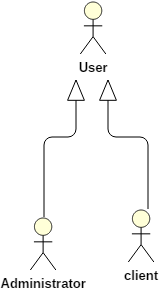
\includegraphics[width=4.75cm,height=4.5cm]{chapter3/actors.png}
\end{center}
\caption{Inheritance Relationship between Actors}
\label{actors}
\end{figure}


\subsection{Functional requirements}

The delivered application consists on designing and implementing Client / Server application that should satisfy the specific functionalities listed below:
\begin{itemize}
\item The system must offer to the user the possibility to load big data from different sources into HDFS. 
\item The system must engineer the best implementation of the required algorithms in order to perform the best execution time and memory management.
\item The user is not coming from An IT background; all command lines should be hidden behind a Graphical User Interface. 
\item The system allows user to apply, on large volume of data, several data mining algorithms such as:
\begin{itemize}
\item Principal components analysis 
\item Linear Model
\item K-Means
\end{itemize}
\item The User should be able to visualize algorithm results in different interactive forms (Charts, Graphics, data visualizations, grids …)
\item The application should provide a users management feature in order to affect different roles for every user category.
\item The application should provide for the administrator user the ability to log every operation lunched by the client. This functionality enables reporting issues.
\item This application should offer the ability for every client to ask for a registration. After administrator permission, he would be able to access and process algorithm on his loaded data.
\end{itemize}
\subsection{Non-functional requirements}

While achieving the functional requirements, the solution should satisfy the following non functional requirements:
\begin{itemize}
\item \textbf{Scalability:} The modularity and extensibility of the application architecture in case of the addition of new features or new algorithm. In our case, when the size or volume of data becomes larger or the number of servers increase, the application should guarantee a regular behaviour. We can also add new algorithms in case of necessity. 
\item \textbf{Ease of use:} As users are almost from a non-IT background, the application must have a user-friendly and ergonomic interface.
\item \textbf{Security:} The data storage should be far from being accessed by an unwanted user. Every operation of access should be preceded by an authentication. Data storage servers should be able to provide availability of the data when required.
\item \textbf{Robustness :} Robustness is the system's ability to cope and deal with errors that may occur during the system's execution. It is an important criterion to the system. In fact, the application should ensure a good error management when displaying data or processing. Accidents
like a server crash or failure should be handled in a safe way and error. Moreover, error messages should be precise and correct.

\item \textbf{Documentation:} The solution should be well-documented in order to provide the best use for the costumer.
\end{itemize}
\section{Requirement Specification}
To have a better understanding of the required needs, we will model them in a formal way using use case and activity diagrams.
\subsection{System Use Case}
The use case diagram captures the behaviour of a software system. This diagram describes
the various actions, which can be made by an outside user. It splits the feature of the system into coherent units, the use cases, having a sense for the actors.\\

The figure \ref{user} shows the general use case diagram that includes the common functionalities for all components.\\

In order to clarify the previous diagram, we present a detailed description of the use case in the table \ref{description}.
\begin{figure}[H]
\begin{center}
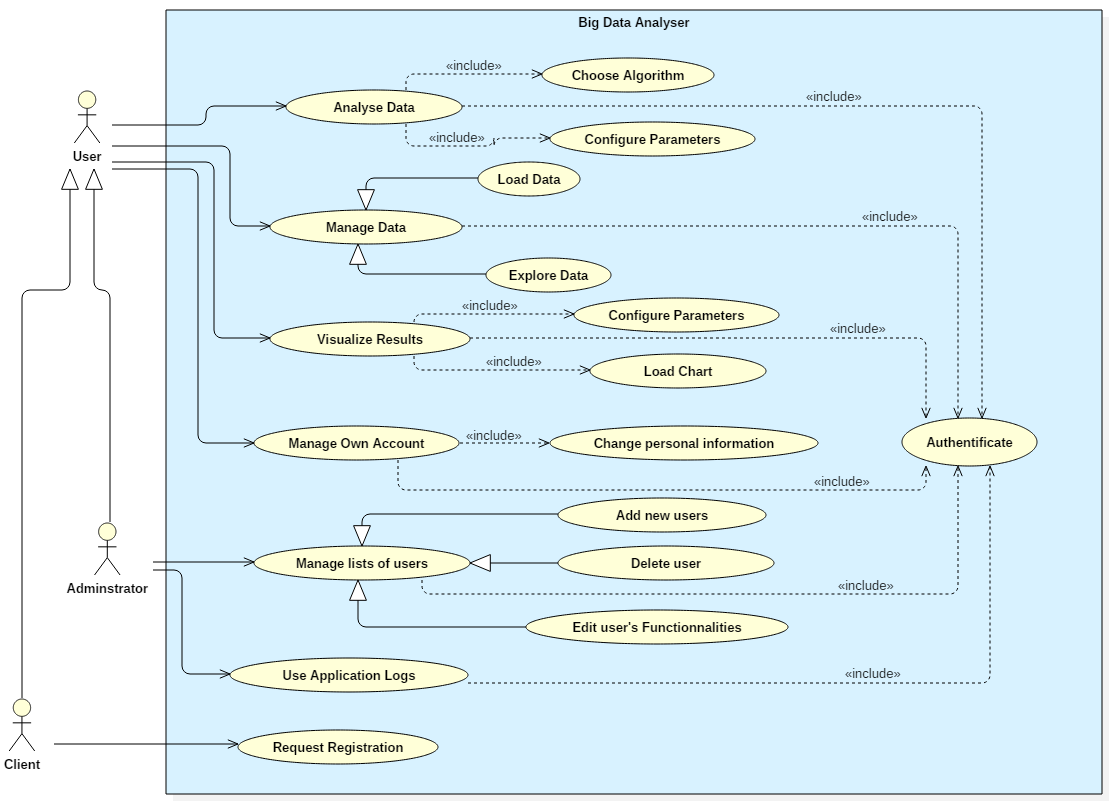
\includegraphics[width=17cm,height=16.3cm]{chapter3/userrusecase.png}
\end{center}
\caption{General Use Case}
\label{user}
\end{figure}

\begin{table}[H]
\caption{Use Cases Description}
\begin{center}
\begin{tabularx}{17cm}{|p{3.5cm}|X|X|}

\hline
	\textbf{Actor} & \textbf{Use Case} & \textbf{Description} \\ \hline
    \multirow{4}{*}{User}&Analyse  Data&Analyse data is the first main feature that should be provided. \newline A user should choose as a first step which algorithm to run. Then as a second step, the user should configure algorithm parameters before running it. \newline This use case must be preceded by an authentication. \\ \cline{2-3}
    &Manage Data&Mange large scale of data is the second main feature that should be provided. User should be enabled to load data and explore its emplacement. \newline This use case must be preceded by an authentication.\\ \cline{2-3}
    &Visualize Results&Visualize results is also a main feature of the application. Result are sort of graphs and charts. Therefore, user should configure parameters (e.g. choosing axes) and then load chart. \newline This use case must be preceded by an authentication.\\ \cline{2-3}
    &Manage Account&The application must enable users to manage their own information in their accounts (e.g. password, user name ..). \newline This use case must be preceded by an authentication. \\ \hline
    
     
    \multirow{2}{*}{Administrator}&Manage list of users&The Administrator has exclusively the right to confirm new users’ right to access to their accounts after verifying their identity. \newline As being a critical use case, this operation must be preceded by authentication.\\ \cline{2-3}
    &Use Application Logs&Each operation processed must be logged in a way that enables the administrator to control application operations. \newline This use case is very important in order to register traceability of the processed operations which make reporting issues easier and more efficient. \newline This use case must be preceded by an authentication. \\ \hline
    
    
    Client&Request Registration&As a first step to interact with our application, a user should fill a form on which he describes his identity.\newline After this step, he waits for the administrator confirmation to access the application.\\
    \hline
    
\end{tabularx}
\end{center}
\label{description}
\end{table}


\subsection{Activity Diagram}
\subsubsection{Administrator Activity Diagram} 
The figure \ref{act1} shows an activity diagram that describes the flow of control relative to the \textbf{administrator}. It illustrates the main possible activities, actions and decisions made through interaction with the system.\\
  
When the administrator open the application on his web browser, he receives first the login page. He types his login name and password; if they (login + password) are correct, he will have access to the application. Otherwise, his request will be rejected and he will redirected again to the login page again. After getting the access to the application, the administrator will main menu. The provided options are \textbf{Manipulate Data}, \textbf{Choose the Manage List of users} and \textbf{Choose the Consult Application Log option}. If the user chooses the \textbf{Manage List of Users} option, he will be asked either to \textbf{Add new user}, \textbf{Delete existing User} or \textbf{Edit user features}.


\begin{figure}[H]
\begin{center}
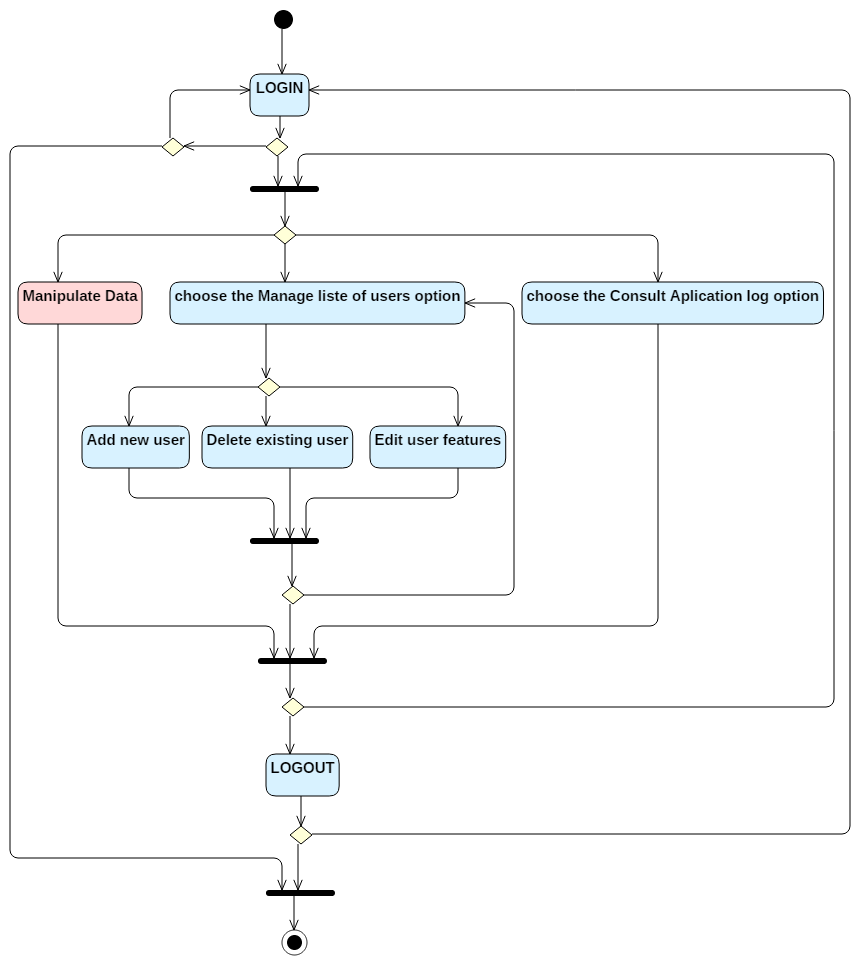
\includegraphics[width=17cm,height=16.7cm]{chapter3/administrator.png}
\end{center}
\caption{Administrator Activity Diagram}
\label{act1}
\end{figure}


\subsubsection{Client Activity Diagram}


The figure \ref{act2} shows an activity diagram that describes the flow of control relative to the \textbf{client}.\\

As a first step, a client should fill the registration form, providing his personal information. Filling this form is considered as a request to get access to the application. After this step, the client will wait for a confirmation from the administrator; if he get it (the confirmation), he will be able to access after. Otherwise, he will be rejected to fill a request again or quit the system.\\

Getting the confirmation will give the client the ability to login the system, manipulate his own data as much as he wants and then leave by logging out.  

\begin{figure}[H]
\begin{center}
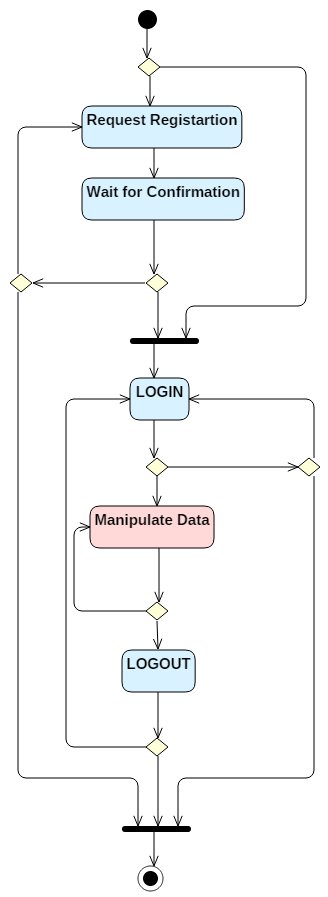
\includegraphics[width=7.5cm,height=17cm]{chapter3/client.png}
\end{center}
\caption{Client Activity Diagram}
\label{act2}
\end{figure}

\subsubsection{General User Activity Diagram}
The figure \ref{act3} shows a general activity diagram that describes the flow of control relative to the common operation for both actors which is: \textbf{Manipulate data}. When the user sits in front of his computer, open the application on his browser he receives, first, the authentication page. He types his login name and password. If it matches together (login + password), the user access to the application. Otherwise, he will redirected to the login page again. After getting the access the application, the user receives the main menu, from which he can choose either \textbf{Manage Data}, \textbf{Analyse Data} or \textbf{Visualize Data}. \\

 If the user chooses the \textbf{Manage Data} option, he will we asked to choose if he wants to load new data or to explore existing data through a file manager. If the user chooses the \textbf{Analyse Data} option, then he is asked which is the appropriate algorithm to run on selected data, configure the algorithm parameters and process it by the end. If the user chooses the \textbf{Visualize Data} option, then he will be asked to fill the configuration form (select result to visualize, select axes …). This step will make loading charts possible. 

After all, the user will have the choice either to to logout from the application or to operate again one of the previously mentioned options.\\


\begin{figure}[H]
\begin{center}
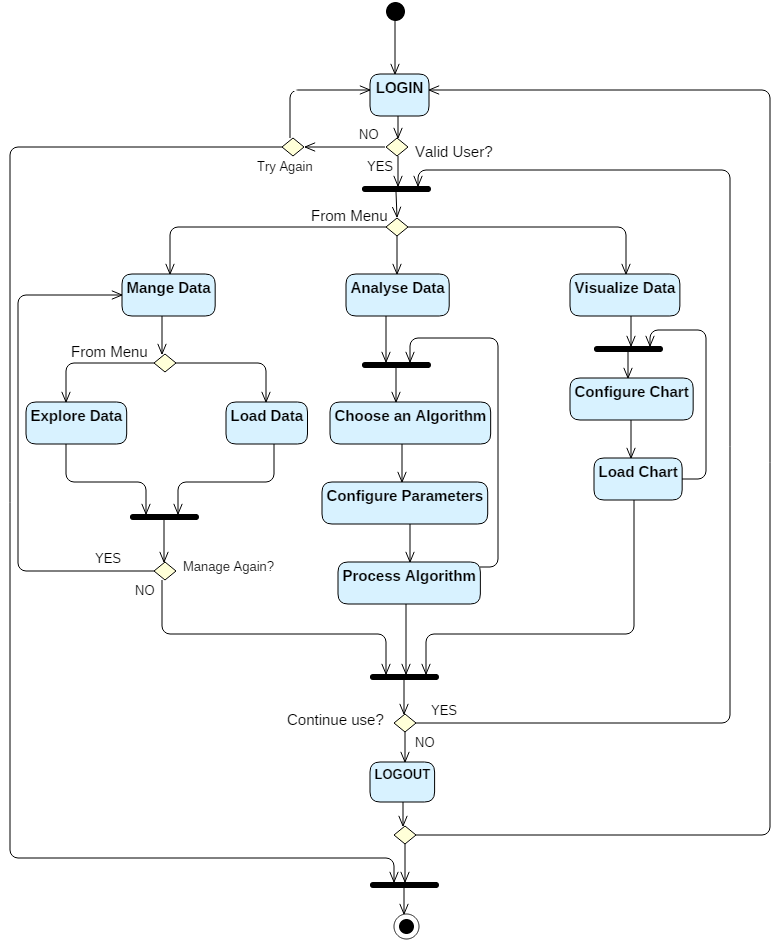
\includegraphics[width=17cm,height=15cm]{chapter3/activity.png}
\end{center}
\caption{General user Activity Diagram}
\label{act3}
\end{figure}




 
\section*{Conclusion}

In this chapter, we have presented the requirements and the needs of the system and its users. We have first identified the actors of our system and explicit the functional and non-functional requirements. Then, we have detailed these needs by specifying, in more details, the features expected through a detailed use case and activity diagram. Thus, we can begin the design phase, which will be the purpose of the next chapter.
